\section{Reverse Engineering the Movement
Machine}\label{reverse-engineering-the-movement-machine}

\{\#sec:physiology\}

\begin{quote}
\emph{Even a simple movement is a global body event.}

--- Bizzi \& Ajemian, \emph{2020}
\end{quote}

\subsection{Motor Units to Muscles}\label{motor-units-to-muscles}

The quantum of motor output is the motor unit (MU), defined as a single
motoneuron axon and the set of junctions the terminals of its axon
branches form with one or more muscle fibers. The MU provides the motor
system with spatial redundancy at the muscle level: multiple muscle
fibers contract due to a single alpha motoneuron (AMN) spike in the
spinal cord's ventral horn, and multiple AMNs may overlap in their
innervations. The forces produced by motor units span several orders of
magnitude, though most units produce very small forces. Here we find
temporal redundancy: in order to produce movements, MUs combine to
generate a range of
forces{[}@fuglevandMechanicalPropertiesNeural2011{]}. Since the
innervation ratios of muscles in the forearm and hand are relatively
small compared to more proximal muscles (which contain thousands of
MUs), the logarithmic recruitment and redundancy of motor units enables
the hand to produce movements with very fine spatiotemporal resolution.

Muscle fibers are contained within muscle compartments, and each muscle
may have one or more compartments. The fingers of the hand are extended
by the extensor digitorum (ED) which contains four compartments, one for
each of the tendons the muscle produces. Each tendon connects to the
three metaphalangeal joints of each digit. The fingers are flexed by two
muscles, the flexor digitorum superficialis (FDS) and the flexor
digitorum profundus (FDP). Like the ED, these muscles produce four
tendons, one to each finger from each of their four compartments. As
such, one must coactivate these agonist and antagonist muscles in order
to extend or flex a single finger in
isolation{[}@fuglevandMechanicalPropertiesNeural2011{]}. Adduction and
abduction of the fingers is produced by the 19 intrinsic muscles of the
hand, each of which has their origin and insertion points within the
hand itself{[}@vanduinenConstraintsControlHuman2011{]}. The intrinsic
muscle tendons form a kind of network around each of the digits. The
human hand, thumb, and forearm system contains more than 30 muscles and
at least 20 degrees of freedom are theoretically available for
actuation. However, due to biomechanical coupling, the effective degrees
of freedom is presumably less than 20.

This structure exists in order to facilitate the acquisition of new
skills and the generalization of existing skills to new contexts. While
the anatomy of the hand and forearm presents constraints on movement,
the system remains capable of producing an incredible variety of
movement
patterns{[}@yanUnexpectedComplexityEveryday2020;@Basmajian1963{]}\footnote{In
  a classic study, Basmajian and colleagues showed that it is possible
  to activate single motor units in the thumb abductor.}. The structure
of the neuromuscular system that underlies this variety offers many
clues as to the relevant computations required for dexterous movement.
In \{+@fig:low\_variance\_PCs\}, Yan et al.~show how even low-variance
principle components of joint kinematics during object grasping and ASL
signing display correlational structure and not merely noise. That is,
the production of hand movement is highly task-specific, where
individual tasks are linked to bespoke muscle activations patterns.

\begin{figure}
\phantomsection\label{fig:low_variance_PCs}
\centering
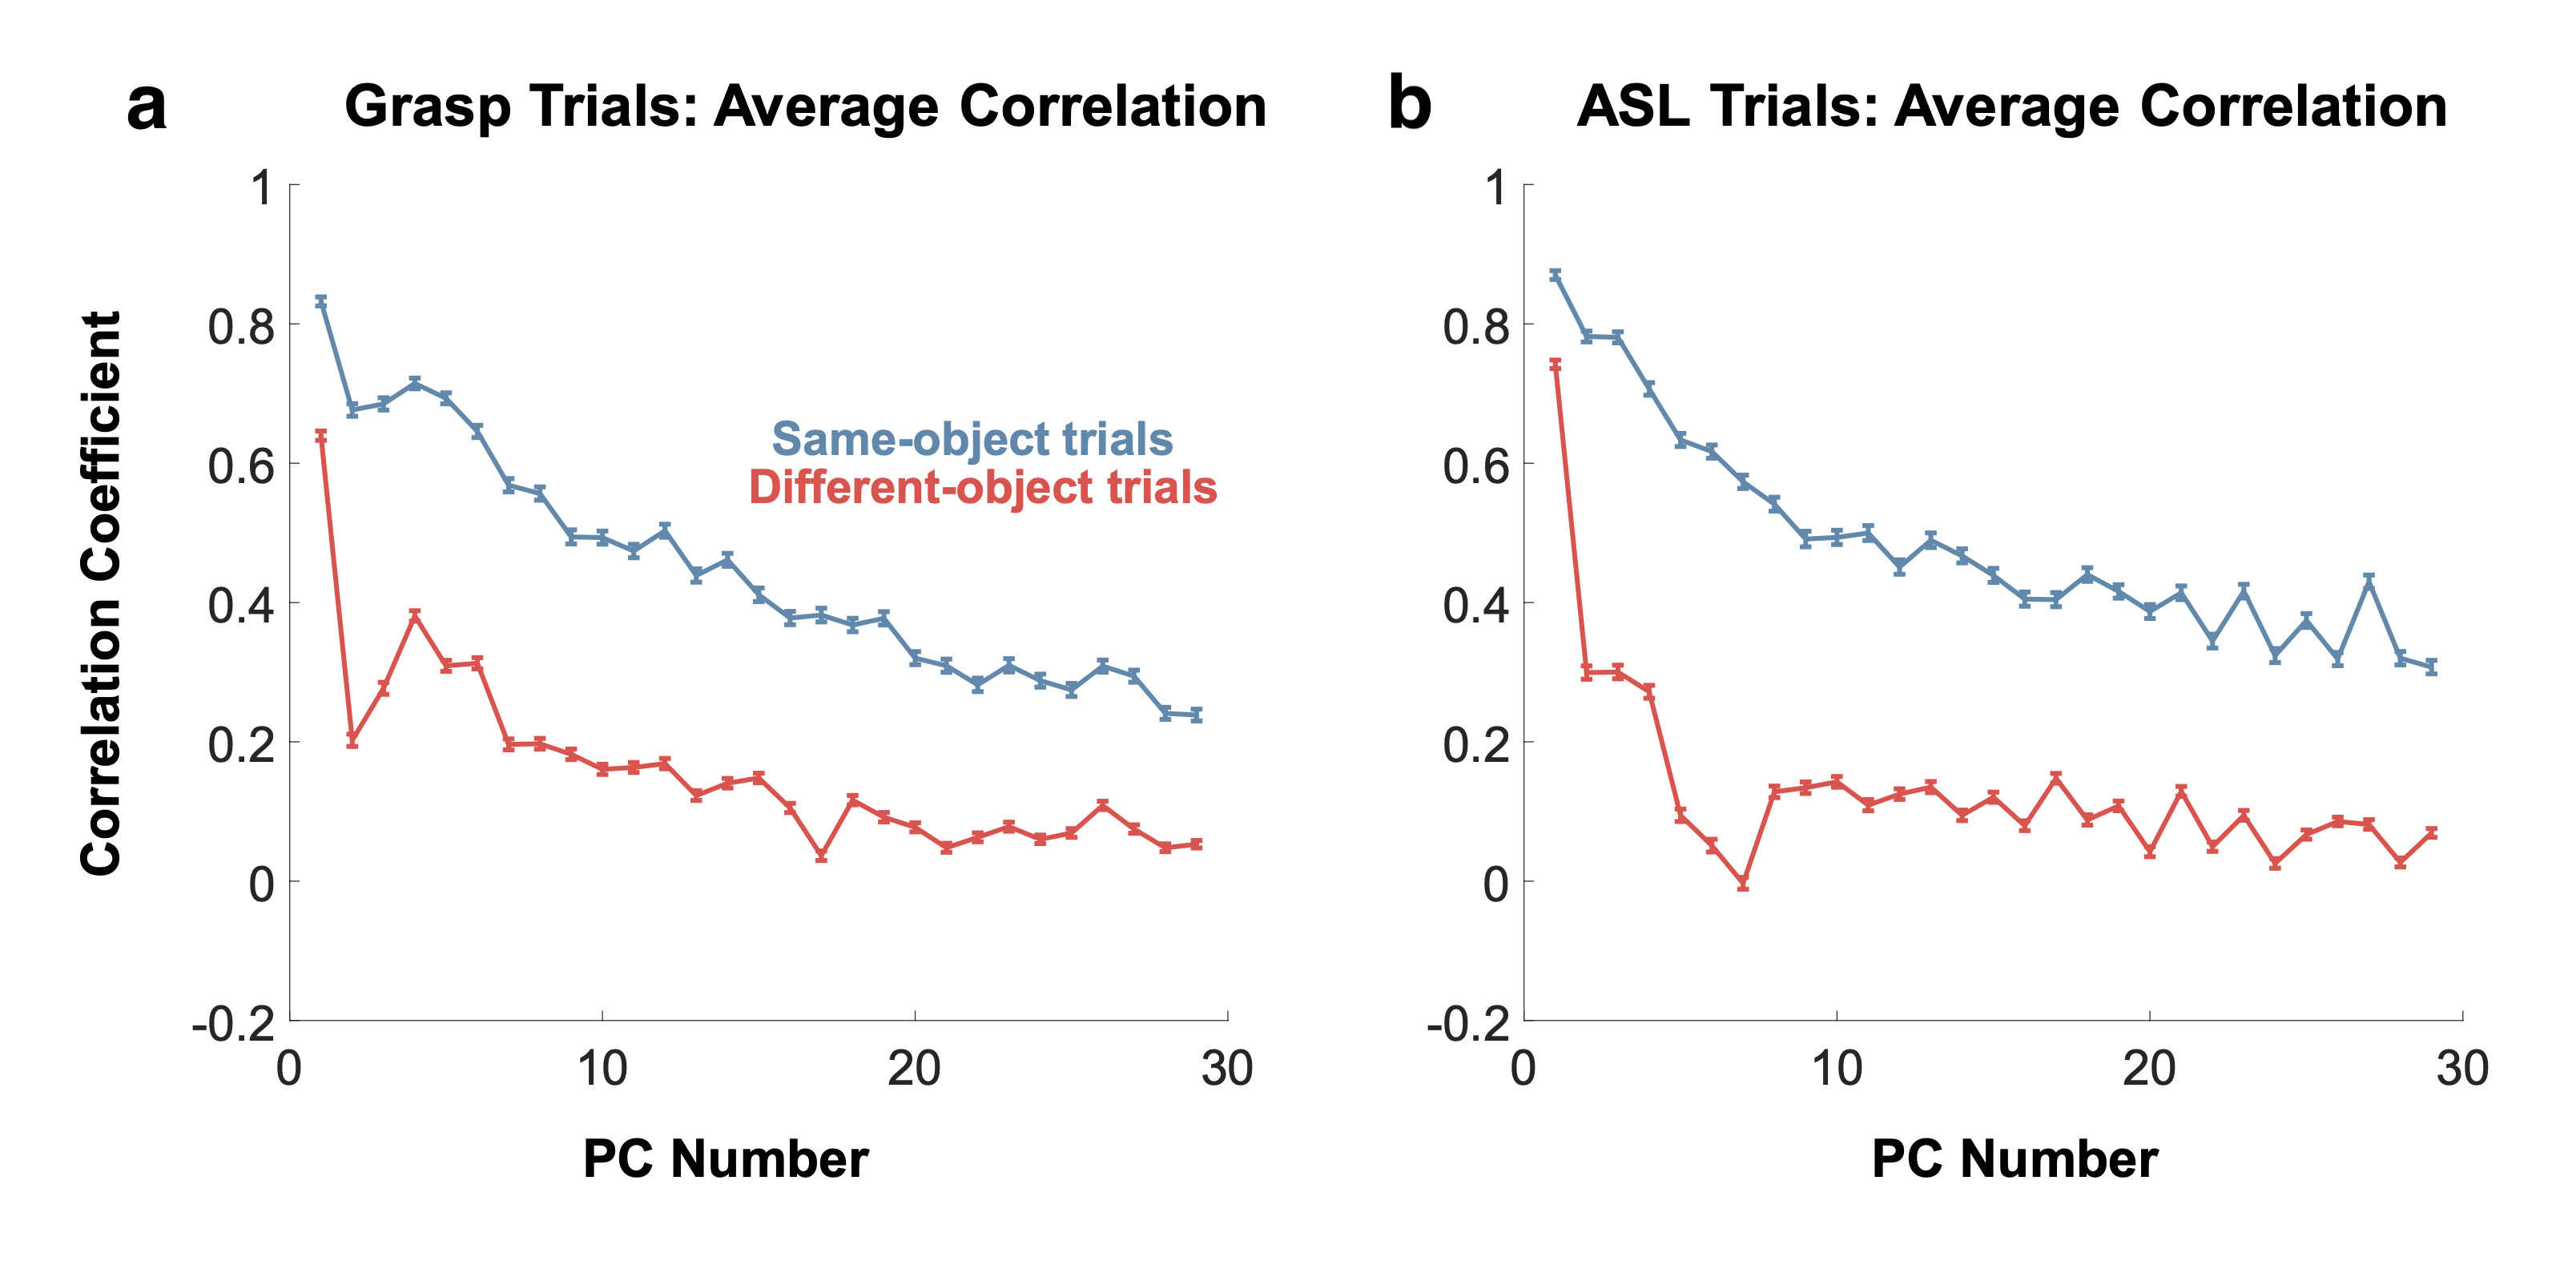
\includegraphics[width=1\textwidth,height=\textheight]{../images/physiology/background/low_variance_PCs.png}
\caption{Taken from Yan et al.~2020. Plots show mean correlations
between hand joint kinematic trajectories during grasp trials with the
same (blue) and different (red) objects (a) and ASL signs (b) projected
onto the same principle components. Correlations are averaged across 8
subjects. Within-object and within-sign correlations are systematically
higher than their shuffled counterparts. Error bars denote SEM. This
data supports the idea that low-variance components of kinematics data
contain task-specific structure rather than merely reflecting noise.
This is encouraging for our experiments, which hope to extend this idea
into careful analyses of task specific features of EMG data across
learning and in response to perturbations.}\label{fig:low_variance_PCs}
\end{figure}

\subsection{Coordinative Structures}\label{coordinative-structures}

Many studies have contributed to the concept of synergies as a
hard-wired organizing feature of the motor
system{[}@mussa-ivaldiMotorLearningCombination2000,@DAvella2003{]}.
However, these works tend to extrapolate from non-primate preparations,
particularly in the frog, and use tasks which are inherently
low-dimensional to explain covariance structure in primate and human
kinematic and electromyography
data{[}@giszterMotorPrimitivesNew2015;@gao2017{]}. That said, it would
be foolish to deny the existence of synergistic muscle coactivation even
at the structural level. Careful studies of force control by the
fingertips present a complex story of dimensionality of control in this
regime{[}@raczSpatiotemporalAnalysisReveals2013{]}. Constraints exist in
the architecture of the hand as well as its control system, though we
maintain that concept of synergies, especially in the context of
dexterous movement, is often presented as an oversimplification rather
than a mere simplification. We believe the story of the hand is more
complex.

Studies have attempted to quantify the number of effective degrees of
freedom of the hand with various methods. This has primarily been taken
to be the number of linear features which contain a desired level of the
original signal variance, where the signal is the joint angles of the
hand engaged in various
behaviors{[}@Ingram2009;@TodorovDimensionality2005{]}. These methods
have resulted in roughly 8 linear features of hand kinematics to solve a
variety of tasks, with subtleties found in inter-task and inter-subject
variations. Note that the motor repertoire is hardly high-dimensional
when compared to the dimensionality of the visual feature extraction
system{[}@yanUnexpectedComplexityEveryday2020{]}. A recent study found
that low-variance linear, kinematic components displayed significantly
higher correlation within condition (e.g.~grasp of a specific object)
than across condition. This suggests that these components carry
task-dependent information rather than condition-independent,
task-irrelevant noise{[}@yanUnexpectedComplexityEveryday2020{]}. This
suggests that the control of the hand is more nuanced than a set of
fixed synergies.

What Bizzi and colleagues call ``the problem of supraspinal pattern
formation''--how synergies are activated through time-- we argue, in the
context of hand control, is not simplified by the existence of
hard-wired or soft-wired
synergies{[}@bizziMotorPlanningExecution2020{]}. Rather, the CNS
produces control signals in a range of contexts and in response to
continually changing task demands. Rather than the CNS ``simplifying
movement'' through synergetic action, it is more likely that hand
synergies fall out of a optimization strategy which trades off effort
and accuracy where effort may, in part, correspond to independent
control of individual control dimensions. In this view, synergies,
hard-wired or not, reflect the statistics of the environment in which
movement is
constructed{[}@brutonSynergiesCoordinationComprehensive2018{]}. If we
limit ourselves to synergetic control, then we have simply passed the
problem to a lower-dimensional one of the same fundamental nature.
Neural control of the hand likely contains a spectrum of modularity in
order to maintain its role as a flexible instrument. Synergetic action
is one end of this spectrum resulting from the computations inherent to,
along with the structures of the human movement machine.

\subsection{Fractionating Structures}\label{fractionating-structures}

Just as many muscle fibers may be innervated by a single AMN, up to
thousands of neurons contact single AMNs through monosynaptic
corticospinal, or corticomotoneuronal (CM), connections and other
descending pathways through elaborate spinal circuitry. The hallmark of
CM connections in particular is their influence over multiple muscle
compartments as well as multiple muscles, though typically agonist or
antagonist sets{[}@cheneyFunctionalClassesPrimate1980{]}. This may seem
counter-intuitive as a means to produce individuated movement, but
experimental evidence in primates has shown that the convergence of many
CM collateral fibers onto single AMNs driving the distal muscles in
particular can produce a fine grading of activity over motor units
driving the distal joints. CM cells also appear to play a role in the
inhibition of antagonist muscles prior to contractions required for
movement {[}@griffinMotorCortexUses2020{]}. These findings confirm
theories about the excitatory and inhibitory role of these connections
dating back decades, and combine to suggest that variables encoded in
cortical ensembles are more complex than kinematics or dynamics
alone{[}@cheneyFunctionalClassesPrimate1980{]}.

The CM tract thus acts in coordination with synergistic muscle
activations of the hand to achieve control that is balanced between
modularity and flexibility. Findings suggest that there is a bipartite
structure in human motor cortex driving dexterous control of the distal
part of the upper limb which, it has been suggested, evolved under
pressure to quickly generalize between tasks. This work argues that
these two streams of hand control, namely ``fractionated'' and
``synergistic'' control, may interact to produce versatility, and
balancing these subsystems may be a key part of the optimization
function when learning new
skills{[}@Rathelot2009;@griffinCorticomotoneuronalCellsAre2015;@Takei2017{]}.
This dualism is likely not rigidly dichotomous, but rather a spectrum of
overriding fractionation (so-called ``New M1'') atop a phylogenetically
older system of synergistic
action{[}@dumCorticospinalSystemStructural2011{]}. Griffin and
colleagues found that CM cells are functionally tuned to a muscle's mode
of activity (agonist, antagonist, fixator) to ``bypass spinal cord
mechanisms and sculpt novel patterns of motor output that are essential
for highly skilled
movements''{[}@griffinCorticomotoneuronalCellsAre2015{]}. The hypothesis
stemming from the previously described work is that CM connections
override the ``consolidated'' patterns putatively generated via spinal
interneuron circuitry. The setup devised in our work aims to measure
fractionation by tracing motor unit correlations across learning.
Whether fractionation in our experiments is due to the CM pathway can
only be speculation, but our work may provide direction for future
studies pairing intracortical recordings with careful electromyography.

\subsection{Supraspinal Motor Maps}\label{supraspinal-motor-maps}

It is known from recent work that primary motor cortex (M1) is not an
isolated movement-generating dynamical system, but rather a node in the
network of a feedback-modulated, distributed movement
machine{[}@sauerbreiCorticalPatternGeneration2019{]}. Thinking of the
structural architecture of M1 as an input-driven system with outputs
along a spectrum of modularity from synergistic to fractionated, we can
ask what kind of functional architecture might have evolved in the
neuromuscular controller? Graziano and colleagues found that 500ms
electrical stimulation to M1 reliably produced stereotyped movements in
primates{[}@graziano2006{]}. These movements appeared to produce
goal-oriented actions pulled out of other contexts such as bringing food
to the mouth, and seemed to be arranged on the cortical sheet
topographically in terms of spatial endpoints rather than as a
humunculus. Graziano refers to this as the cortical ``action map'', that
these stimulations tapped into the control mechanisms of the primate's
motor system{[}@grazianoIntelligentMovementMachine2009{]}. These results
has recently been confirmed by optogenetics work in marmosets and
macaques {[}@ebina2019;@watanabeForelimbMovementsEvoked2020{]}.

The motor map concept suggests interpreting activity in M1 as a field of
feedback control microcircuits, integrating and transforming inputs,
both internal and external, to sculpt ongoing
movement{[}@wiltschkoMappingSubSecondStructure2015{]}. This is in
accordance with the idea that there is a structural hierarchy in M1
covering a spectrum of movement modularity. These ideas together form a
picture of the motor system as a structural scaffold upon which
behaviorally relevant feedback mappings from cortex to the spinal cord
are continuously activated and modulated based on information and
estimates about the periphery. In this view, the encoded variables of
interest depend on the goals, context, and perturbations of the intended
movement. \{+@fig:strick\_graziano\} shows Graziano et al.'s stimulation
results, what might be termed a functional view of the cortical motor
system, next Strick er al.'s described above clarifying the structural
view of modularity in this system.

\begin{figure}
\phantomsection\label{fig:strick_graziano}
\centering
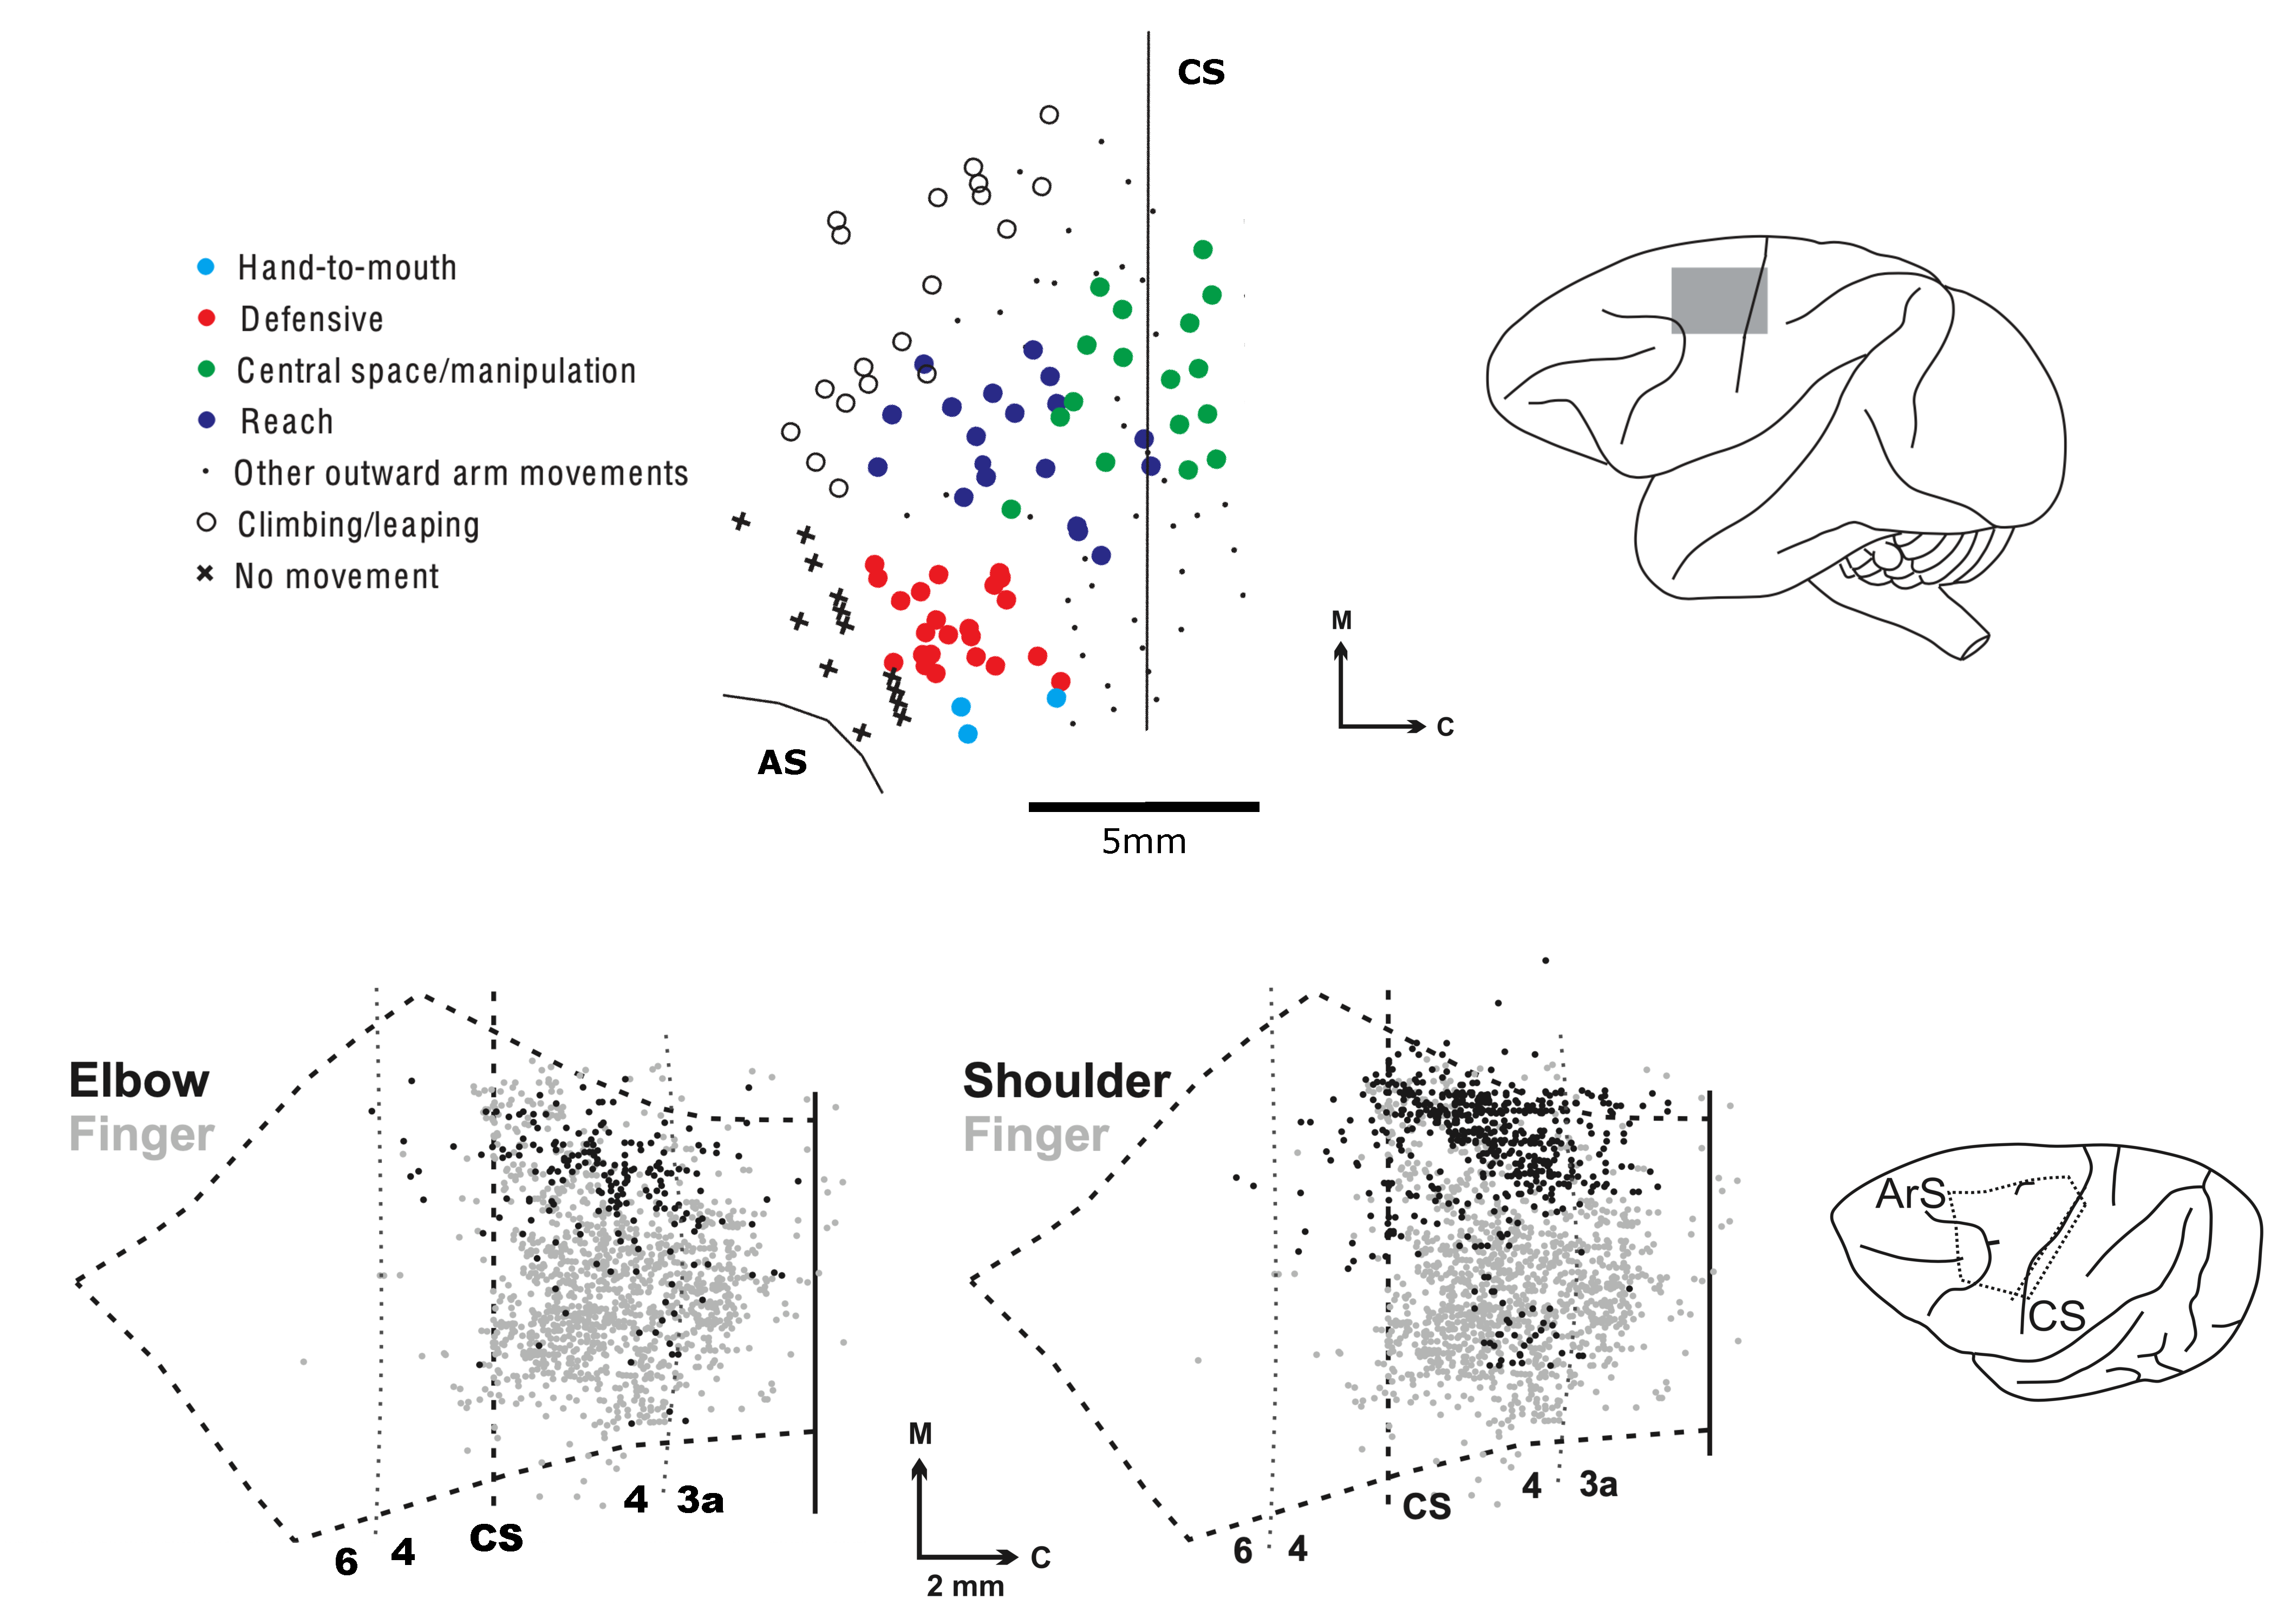
\includegraphics[width=1\textwidth,height=\textheight]{images/physiology/strick_graziano/strick_graziano.pdf}
\caption{Similarities between electrical stimulation on behavorial
timescales and rabies tracing identification of CM cells. CM cells are
largely confined to the caudal half of M1, while this region tends to
evoke complex manipulatory movements when electrically stimulated. (Top
Left) Corticomotoneuronal (CM) cells traced using rabies from muscles of
the elbow and finger. (Top Right) CM cells traced using rabies from
muscles of the shoulder and finger. (Bottom) Complex movements evoked by
500ms electrical stimulation pulse trains. Adapted from Graziano 2005
and Rathelot et
al.~2009{[}@graziano2005;@Rathelot2009{]}.}\label{fig:strick_graziano}
\end{figure}

Graziano writes:

\begin{quote}
``The usefulness of a feedback-dependent mapping from cortex to muscles
is that it can in principle allow neurons in motor cortex to control a
diversity of movement variables, such as direction, speed, hand
position, or posture that transcend a fixed pattern of muscle
activation. If the network receives feedback information about a
specific movement variable, then it can learn to control that
variable.''
\end{quote}

Muscle activity is, in this sense, a readout from a network transforming
state-dependent inputs into movement goals. Rather than choosing muscle
patterns in reconfigurable blocks, it creatively constructs and sculpts
movement. The hierarchy of the motor system may not be rigidly organized
around a particular set of variables. As shown in
\{+@fig:motor\_system\}, many loops exist connecting cortex with the
spinal cord, the cerebellum, the basal ganglia, and the sensorimotor
periphery. Each of these loops contributes information for the flexible
activation of the relevant action maps. Put simply, prevailing evidence
suggests that cerebellar loops provide predictive state information
while basal gangliar loops provide state and/or action value
information. Taken together, this work provides an image of the
incredible complexity which generates dexterous movements of the hand.
This is the foundation on which we can work to build experiments which
elucidate the computations involved in the production of skilled
movement. We aim to connect our results back to what is known about the
system we are attempting to reverse-engineer in order to inspire future
inquiries into the inner workings of the movement machine.

\begin{figure}
\phantomsection\label{fig:motor_system}
\centering
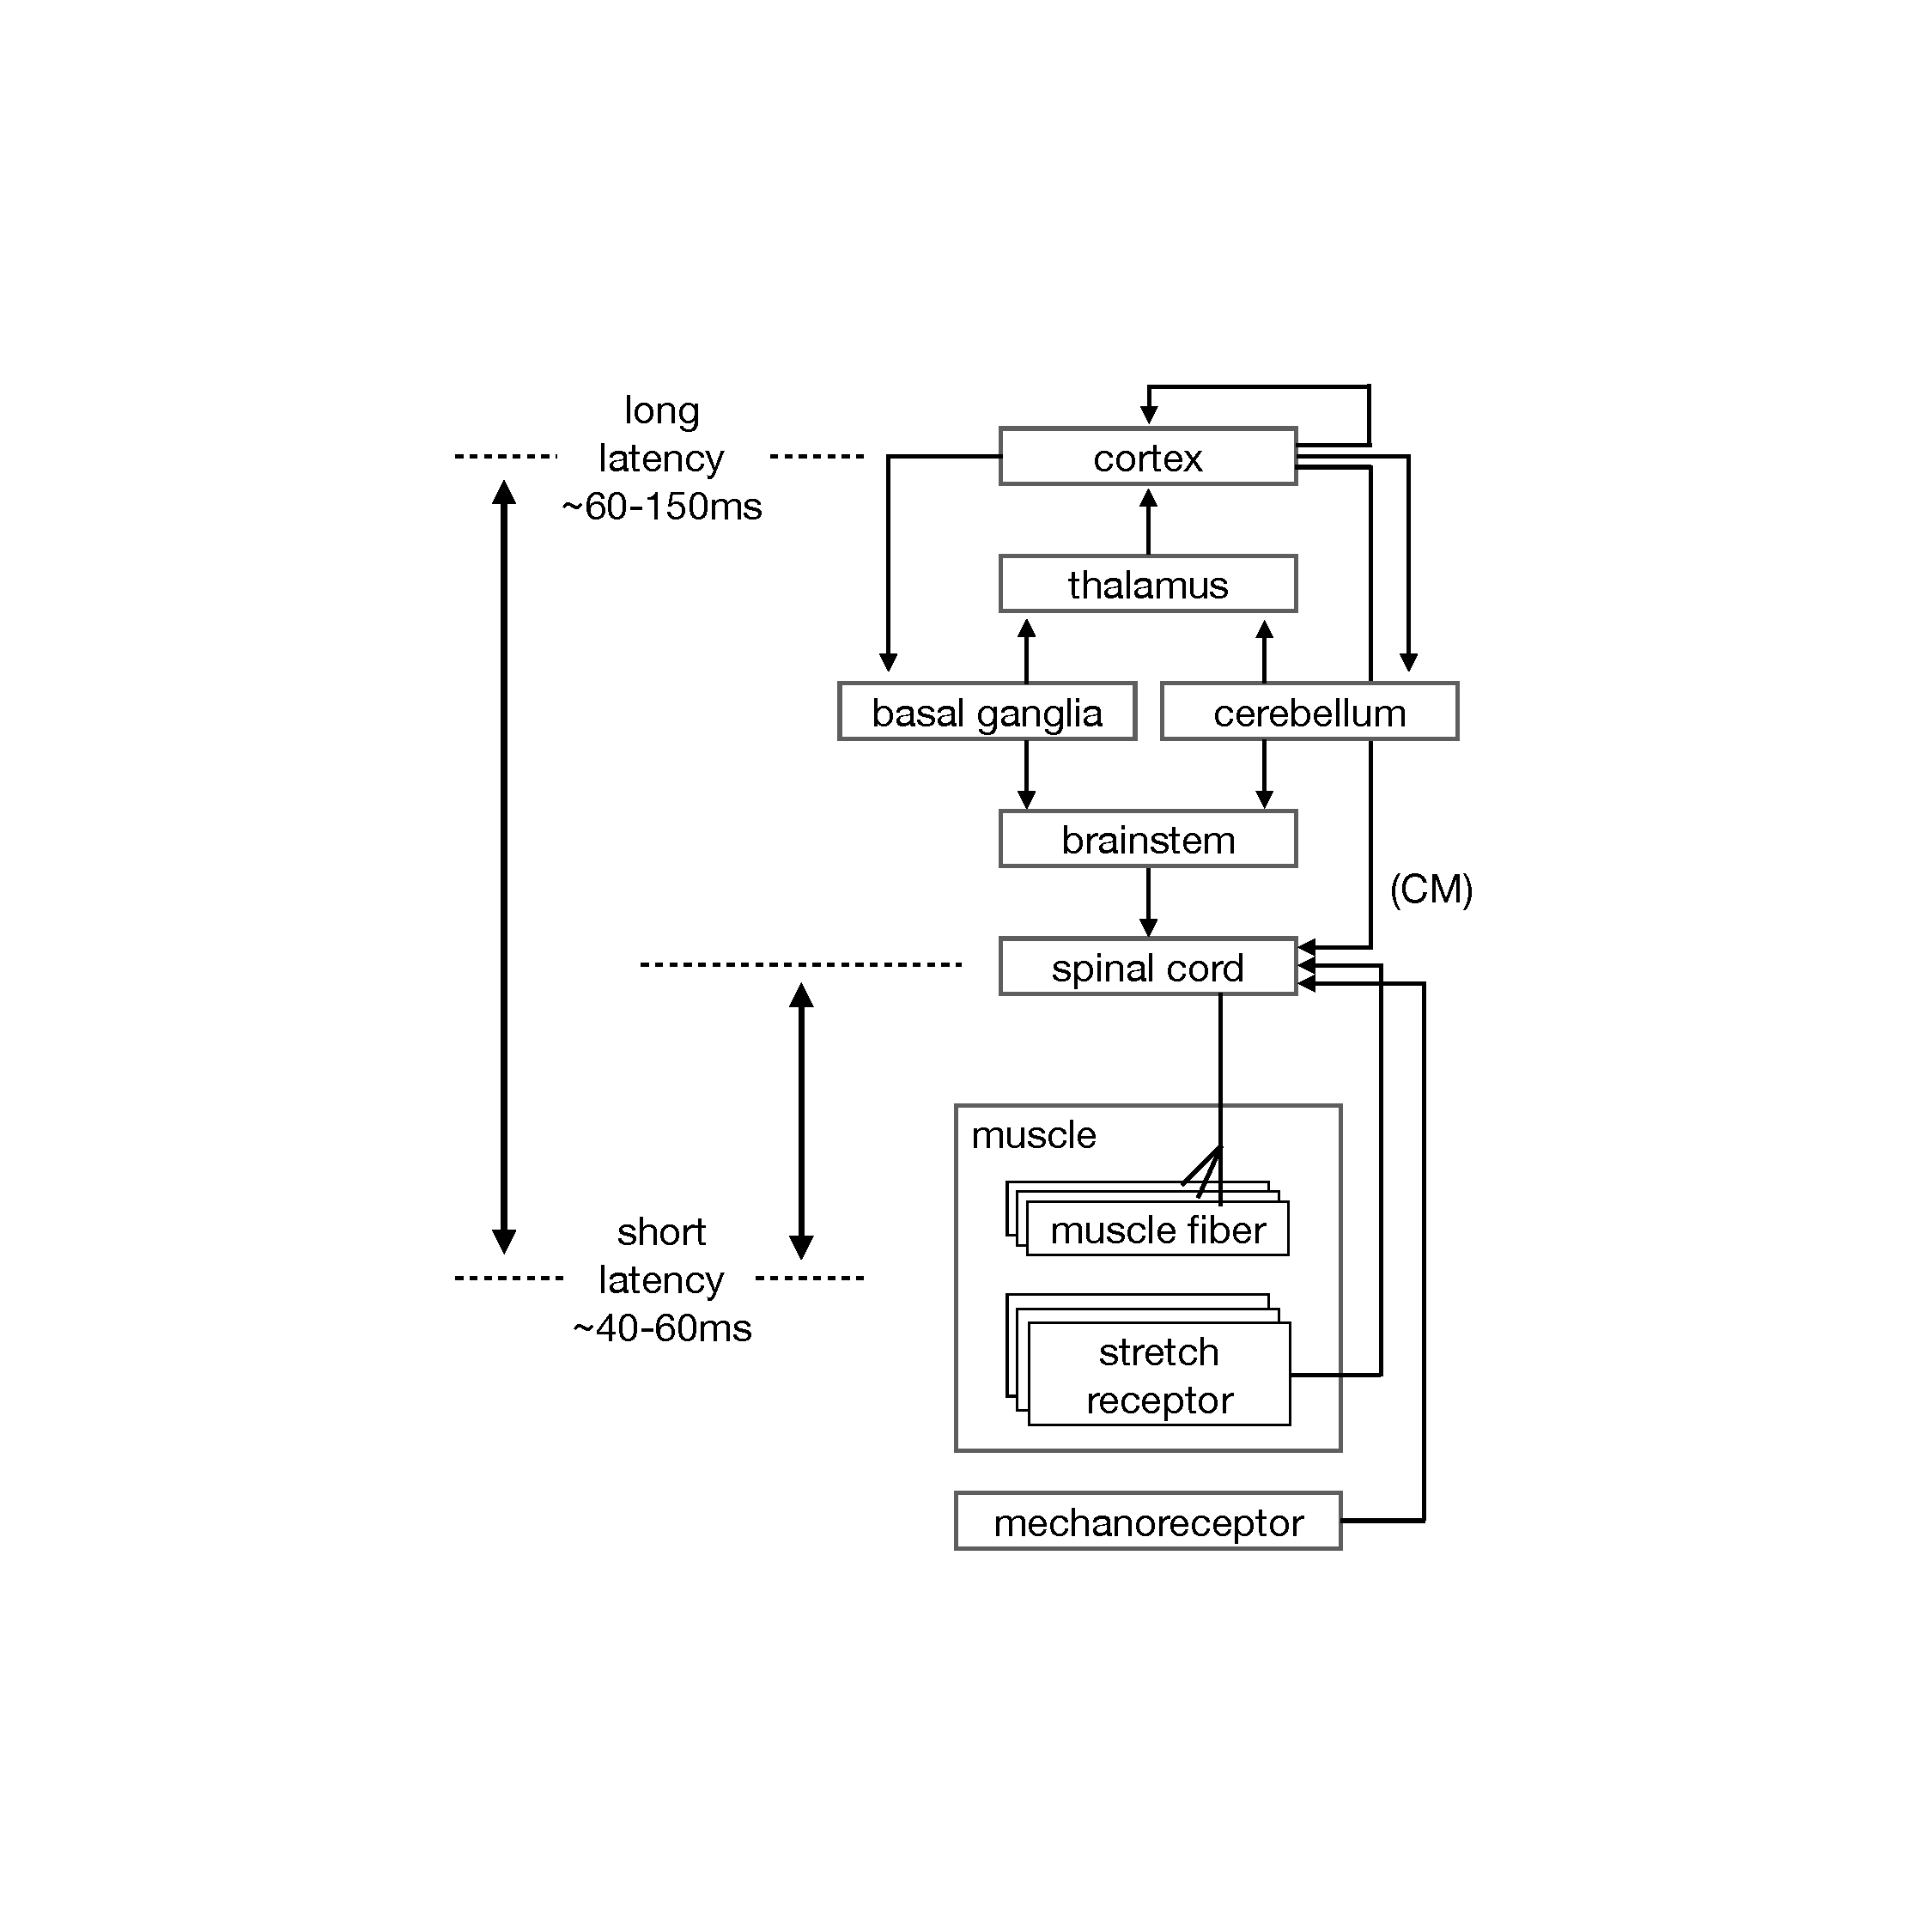
\includegraphics[width=1\textwidth,height=\textheight]{images/physiology/motor_system/motor_system.pdf}
\caption{Overview sketch of the motor system depicting the the
redundancy of the system both hierarchically (multiple muscle fibers are
innervated by the same motor neuron, many motor neurons innervate the
same muscle) as well as heterarchically (parallel spinal,
corticomotoneuronal, cerebellum, basal gangliar feedback loops).
Parallel reflex responses can be classified as long latency
(approximately 60-150ms) and short latency (approximately 60ms). We hope
to consider the parallelism and redundancy of the motor system to
inspire our data analyses and models of motor
computation.}\label{fig:motor_system}
\end{figure}

\subsection{John Rothwell and Jens Bo Nielson: Voluntary
Control}\label{john-rothwell-and-jens-bo-nielson-voluntary-control}

\begin{quote}
In the vast majority of cases, cortical inputs fi rst contact
interneurones which then relay the commands to motoneurones. Since the
same interneurones also receive con -tinuous input from sensory
receptors (and hence might be thought to participate in spinal refl
exes) as well as from interneurones from other parts of the spinal cord,
this means that by the time cortical input reaches motoneurones it has
been fi ltered by multiple lower level systems. In higher primates and
in man, cortical input can access some motoneurones via a special direct
pathway (the corticomotoneuronal pathway), which is often supposed to
play a critical role in volitional movement. However, even if this input
is strong (and there is little comparative evidence on this) the
excitability of motoneurones will have been biased by the multiple other
inputs that each one receives. Thus, even this connection does not
guarantee the brain a straightforward control of muscle.
\end{quote}

\begin{quote}
We argue that distributed cortical projections allow for flexibility of
connections between muscle representations, and therefore are critical
to the flexibility of movements unrestricted by postural demands.
Physiologically, the cortex is the main gateway for visual inputs to
enter and infl uence motor control. This is particularly relevant during
reaching with the arm and during the swing phase of gait for the leg. In
both cases, the limbs are relatively free from feedback control from
gravitational and contact force sensors, and can therefore be driven to
a large extent by visual inputs.
\end{quote}

Posture and contact dictates much of corticospinal function, and we
would expect that these demands influence the architecture of the
underlying circuitry. ``Conscious'' control is likely simply the
availability of visual and propriospinal sensation in the course of the
movement.

\begin{quote}
The anatomy and physiology of the {[}corticospinal{]} connections mean
that if a volitional command were formulated in some hypothetical
centre, it would be extremely diffi cult to predict the consequences
with any certainty unless the state of every interposed connection were
known in advance.
\end{quote}

Nielson argues that hierarchy doesn't function straightforwardly, that
all corticospinal loops can be seen as a collection of distributed,
overlapping modulation of motor neuron activity.

\begin{quote}
About 40 percent of the corticospinal fi bers come from the primary
motor cortex, whereas the cingulate and supplementary areas supply only
about 20 percent each and the premotor areas some 10 percent (Lemon,
2008). All of these areas of cortex also project to brainstem areas that
give rise to reticulospinal tracts, giving them an indirect, cortico-
reticulo-spinal route to the spinal cord as well as the direct
corticospinal route. The primary motor cortex is thought to have fewer
of these indirect connections than other motor areas, suggesting that
its output represents the most `favored' cortical access to spinal cord
circuits.
\end{quote}

\begin{quote}
In primates most of the terminations of the corticospinal tract are on
interneurones in the spinal grey matter with a smaller number of direct
monosynaptic inputs to motoneurones, particularly those inner-vating the
distal muscles of the extremities. These connections represent the only
way the cortex can interact directly with the motor apparatus
(corticomotoneuronal connections).
\end{quote}

\begin{quote}
after pyramidotomy {[}\ldots{]} movements remain slower and fatigued
more rapidly.
\end{quote}

This may be connected to synchronization of the CST? synchronous,
driving input for rapid reactions.

\begin{quote}
We do not know the rules that specify spinal organization in any detail.
However, one striking observation is that most of the connections
between sensory input and motoneurone output are indirect, going via
interneurones rather than direct sensory- motor pathways ( Jankowska,
2001; 2008). An obvious exception to this is the monosynaptic connection
between primary muscle spindle afferents and their homony-mous
motoneurones. However, this seems very much to be a special case rather
than the rule.
\end{quote}

\begin{quote}
One advantage of having interposed interneurones is that they are an
effective way of allowing the spinal circuitry to switch between
different states. For example, in the two funda-mental states of stance
and gait, connectivity during posture should be arranged in order to
resist perturbations of the body whereas during gait postural control
must be released and movement allowed. Going from posture to movement
means turning off the connections that assure stability and turning on
those that allow movement. {[}\ldots{]} A second advantage of
interneurones is that they can specialize in producing different
patterns or rhythms of activity. This could be a special property of
individual neurones or a property of an interconnected network of
neurones, such as envisaged for the locomotor pattern generator.
\end{quote}

Drawing a picture where spinal circuits are autonomous, but modulated,
by cortical input.

\begin{quote}
t is a general fi nding that every single interneu-rone receives input
not only from the sensory modality which is the basis for its classifi
cation (e.g.~as a `Ia inhibitory interneurone', `Ib inhibitory
interneurone', `gr. II interneurone' or `fl exor refl ex afferent
interneurone'), but also from a number of other sensory afferent
modal-ities, other interneurones and a number of descending pathways
(e.g.~corticospinal, vestibu-lospinal, reticulospinal).
\end{quote}

\begin{quote}
It is not an unrealistic possibility that spinal interneurones with a
slight turn of events could have been classifi ed based on their
supraspinal input as taking part in different voluntary movements rather
than the current clas-sifi cation based on afferent input as taking part
in different refl ex actions. This was realized already by Sherrington
(1906) more than 100 years ago when he wrote: ``A simple refl ex is
probably a purely abstract conception, because all parts of the nervous
system are connected together and no part of it is probably ever capable
of reaction without affecting and being affected by various other parts,
and it is a system certainly never absolutely at rest. But the simple
refl ex is a convenient, if not a probable, fi ction.''
\end{quote}

\begin{quote}
\textbf{The discharge of every single motoneurone and thus the
activation of every single muscle fi ber is determined by the integrated
depolarization from on average 10,000 synaptic inputs arising from a
number of different sensory modalities, spinal interneu-rones and
supraspinal control centres.}
\end{quote}

\begin{quote}
Cortical input to the spinal cord should be viewed as using or
modulating the output of the spinal circuitry itself. There is no
separation between `spinal refl exes' and `cortical voluntary movement'.
Instead, it is important to focus on how the neuronal machinery in the
spinal cord may provide an extremely fl exible tool for the execution of
voluntary movements.
\end{quote}

\begin{quote}
We hypothesize that there are at least two advantages of cortical
control. The fi rst is adaptability which emerges as a consequence of
the anatomy of the cortical motor representation. The second is
integration of visual input which is particularly important in shaping
the hand to manipulate objects. Individuation and precision are
secondary consequences of this organization.
\end{quote}

Begs the question of a no-visual experiment?

\begin{quote}
EMG recordings show that very short synchronous bursts of activity are
characteristic of many fractionated fi nger movements, such as writing
and tool use {[}\ldots{]} Interposing interneuronal synapses in these
connections would tend to remove synchrony and smooth out the command.
This is indeed what is seen following corti-cospinal lesion (Farmer et
al., 1993). The CM system may thus also be at the heart of human
evolution in view of the evolutionary advantage of being able to throw
something at an animal in order to kill and eat it.
\end{quote}

\begin{quote}
One- third of the cortex, particularly in the parietal and premotor
areas, is devoted to visual processing. A considerable part of this is
used for shaping/orienting our hand in preparation for grasping and
manipulating objects
\end{quote}

\begin{quote}
the motor cortex may differ from the spinal cord in degree of fl
exibility and a larger possibility of integrating visual input, but
otherwise there are no differences between the motor cortex and the
spinal cord circuitries (after all CM cells project to motoneurones and
receive sensory input much like any good old- fashioned interneurone)
that could warrant a signifi cantly different role in our conscious
experience of control of the movements that we perform. What we are
proposing is that it is not the degree of perceived volition which
determines to what extent the motor cortex is involved in a given task,
but rather the need for fl exible visual control.
\end{quote}

\begin{quote}
We hope that we have made it clear that there is little to support this
distinction between automatic and voluntary tasks. We need to consider
the integration between supraspinal and spinal control centers for any
specifi c task in order to understand how that task is controlled by the
nervous system, and try to avoid putting into it volition and voluntary
which in any case are terms that belong in philosophy or in specifi c
inquiries aimed at unravelling the mechanisms of our cognitive abilities
and our conscious experiences.
\end{quote}

Compelling case to look at the entirety of the system, focusing on the
contributions that cause motor neurons to fire.
